\section{Model 1}

The results displayed in this section are for the activation energy
for the fall off reaction in the ozone mechanism. The percentage of
ozone is taken as 40, 46, 53, 75 and 100 percent according to the
experimental data available~\cite{Streng}. Figure~\ref{subfig-1:Raw Chain} and Figure~\ref{subfig-2:Histogram}
shows results for 1e7 MCMC samples and an interpolation surrogate with 1000
points over the range of the prior.
%% We show the raw samples generated by MCMC and plot the
%% histogram for parameter $E_3$.
In Figure~\ref{fig-2:conv_sample},
for constant surrogate size, the number of samples is varied from
1e5 to 1e7 and convergence of the posterior KDE is observed.
%% The plot is done for surrogate
%% size of 1000 and raw chain size of $1e5$, $5e5$ , $1e6$, $5e6$ and
%% $1e7$ is taken.
%
In Figure~\ref{fig-3:conv_surrogate}, the convergence
study is done for an increasing number of surrogate points.
As we increase the number of points in the surrogate, the resulting
posterior KDE
should be very similar for different surrogate sizes. Results are shown for
surrogate sizes of 100, 500, and 1000. For the surrogate convergence
study, $1e7$ MCMC samples are used.
%% For different starting points of MCMC chain, the
%% MAP point of the resulting pdf does not change. The surrogates for
%% individual concentrations are constructed using linear interpolation
%% function. The initial guess for the MAP point is calculated using
%% Nelder Mead optimization technique.

\bigskip

Figure~\ref{subfig-1:mean_1} and Figure~\ref{subfig-2:auto_11} show
mean and autocorrelation plots for the samples in the Markov chain.
The mean plot shows the initial ``burn-in'' period, after which the
mean converges. Further, the autocorrelation plot shows that
more than 50 samples are required to have uncorrelated samples in the
MCMC chain. Thus, the final MCMC chain used in showing the posterior
distribution truncates the burn-in samples and subsamples according to
the correlation length. This process is called ``chain thinning''.
%% It shows us that we
%% should be using at least more than these number of samples for our
%% analysis.
Figure~\ref{subfig-2:final_e3} shows the posterior of
the parameter $E_3$ following the chain thinning procedure. The
following are the moments of resulting posterior distribution:
Mean: 28.3, Std. Dev.: 0.78, Skewness: 0.066 and Kurtosis: 0.035.

\bigskip

Given the final chain of posterior samples, it is necessary to ensure that the samples of the parameter which we
 are drawing are adequately fitting the flamespeed values of the experiment.
Figure~\ref{subfig-1:40_1} through
 Figure~\ref{subfig-5:100_1} illustrate the calculated flamespeed
 using the generated surrogate models for all the
 parameter samples drawn from the final posterior distribution.


%\subsection{Convergence Study: Number of Samples }

% In this section, we see the convergence of the probability distribution as we increase the raw chain sample size. The plot is done for surrogate size of 1000. In this analysis, raw chain size of $1e5$, $5e5$ , $1e6$, $5e6$ and $1e7$ is taken.



%\subsection{Convergence Study: Surrogate }

 %In this section, we see the convergence of the surrogate. As we increase the number of points in the surrogate, results should be close for different surrogate sizes. The plot is done for surrogate size of 100, 500 and 1000. In this analysis, raw sample chain size is $1e7$.



%\subsection{Flamespeed data fit}

 %It is necessary to ensure that the samples of the parameter which we are drawing are fitting the flamespeed values of the experiment. In this section, we calculate the flamespeed for all the parameters drawn using the surrogate generated before. We have taken $1e7$ sample size and calculated flamespeed for different concentrations of ozone.




%\subsection{Mean and Autocorrelation Plots}

% In this section, we show the mean of the samples and autocorrelation plots . The mean plot shows the initial instability due to sum in period of MCMC and after that it remains constant. It shows us that we should be using at least more than these number of samples for our analysis. The last figure shows the histogram and the various parameters of the distribution are Mean:  28.3, Std. Dev.:  0.78, Skewness:  0.066 and Kurtosis:  0.035.






 \begin{figure}[ht]
   \centering
   \subfloat[MCMC raw chain of samples \label{subfig-1:Raw Chain}]{%
     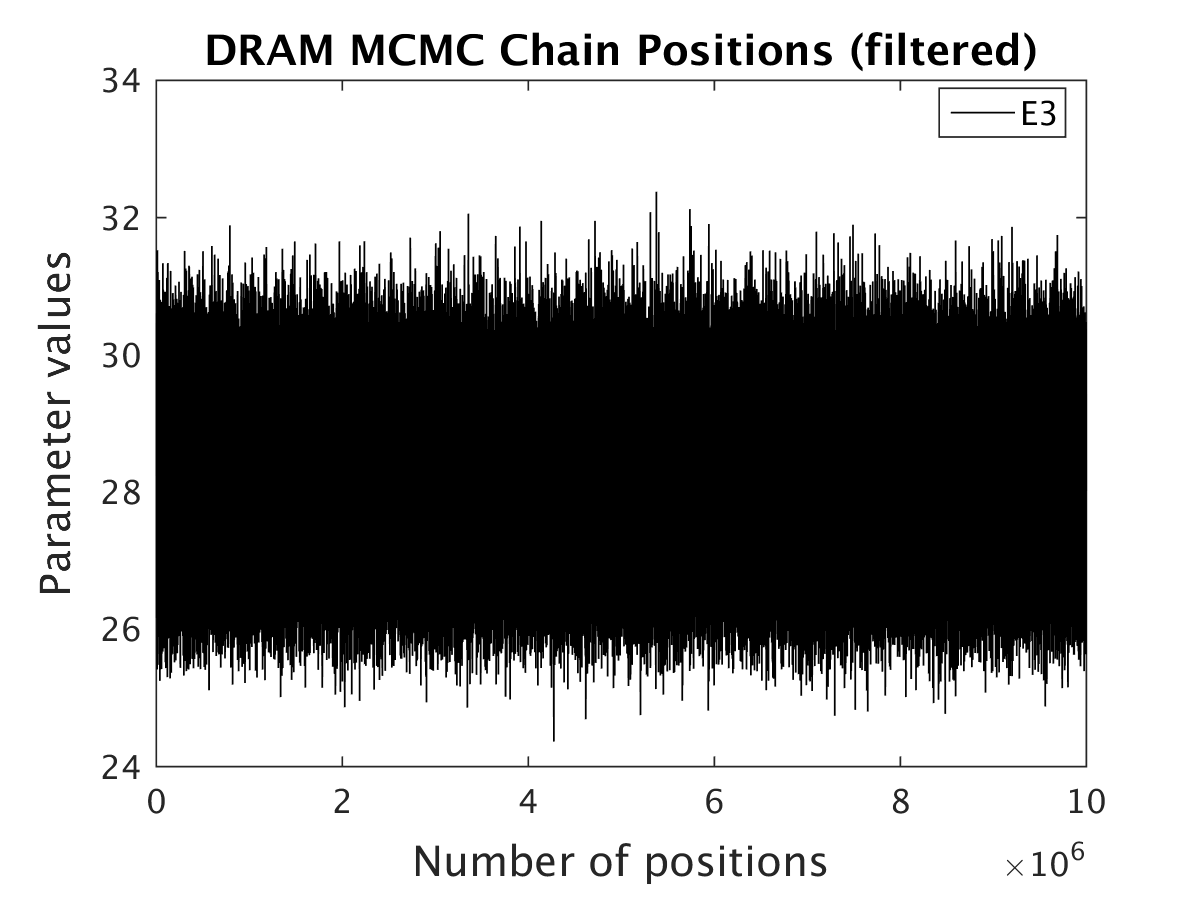
\includegraphics[width=0.45\textwidth]{model_1/simple_ip_chain_pos_filt}
   }
   \subfloat[Histogram\label{subfig-2:Histogram}]{%
     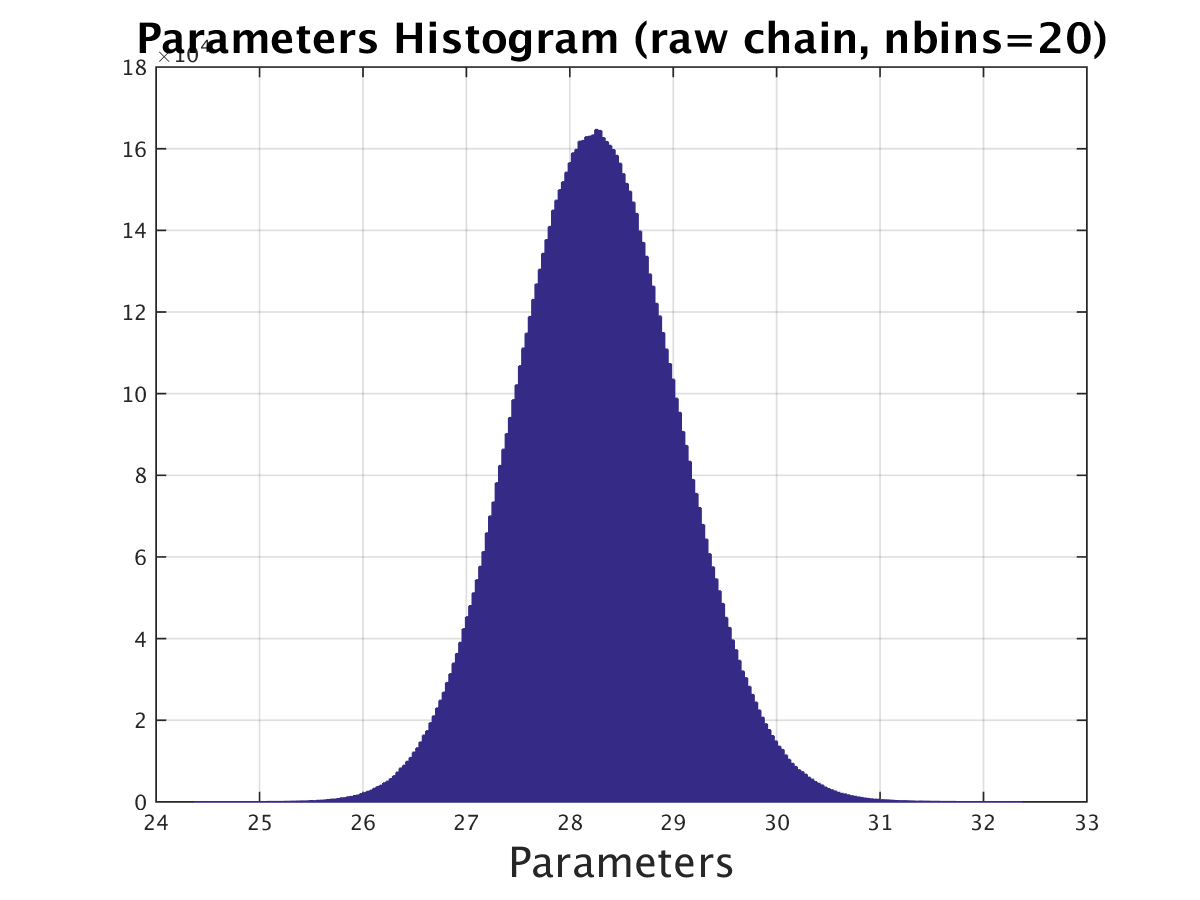
\includegraphics[width=0.45\textwidth]{model_1/simple_ip_hist_raw}
   }
   \caption{MCMC raw chain and histogram for sampling of $E_3$ posterior.}
 \end{figure}




 \begin{figure}[ht]
   \centering
  \subfloat[Convergence of posterior distribution for increasing
    number of MCMC samples.\label{fig-2:conv_sample}]{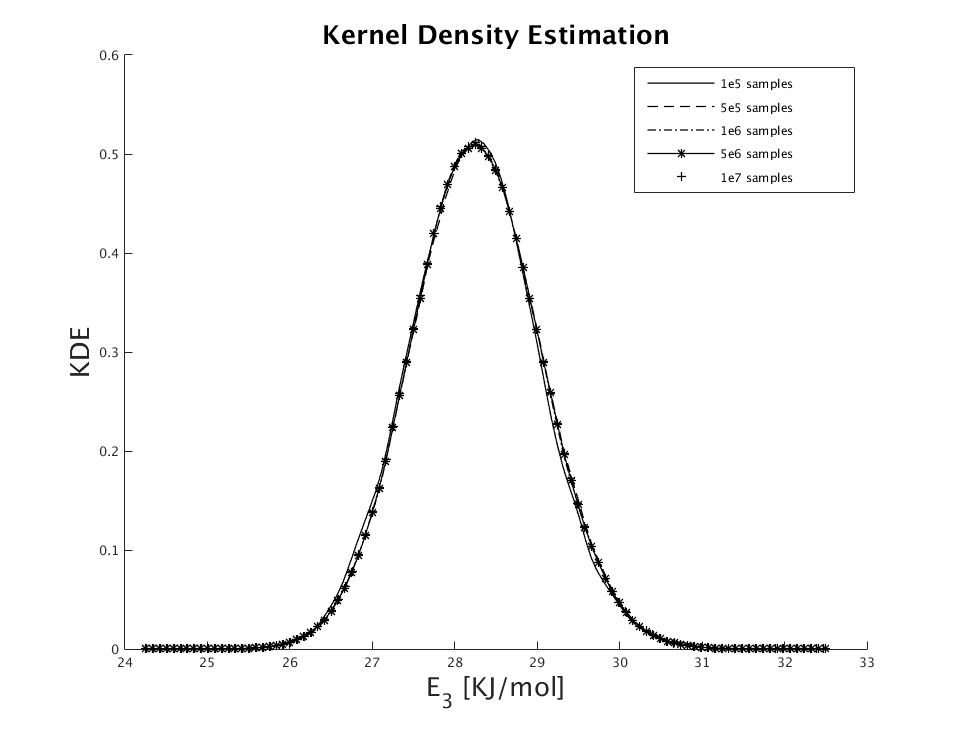
\includegraphics[width=0.45\textwidth]{model_1/sample_conv}}
  \subfloat[Convergence of posterior distribution for increasing
    number of surrogate
    points.\label{fig-3:conv_surrogate}]{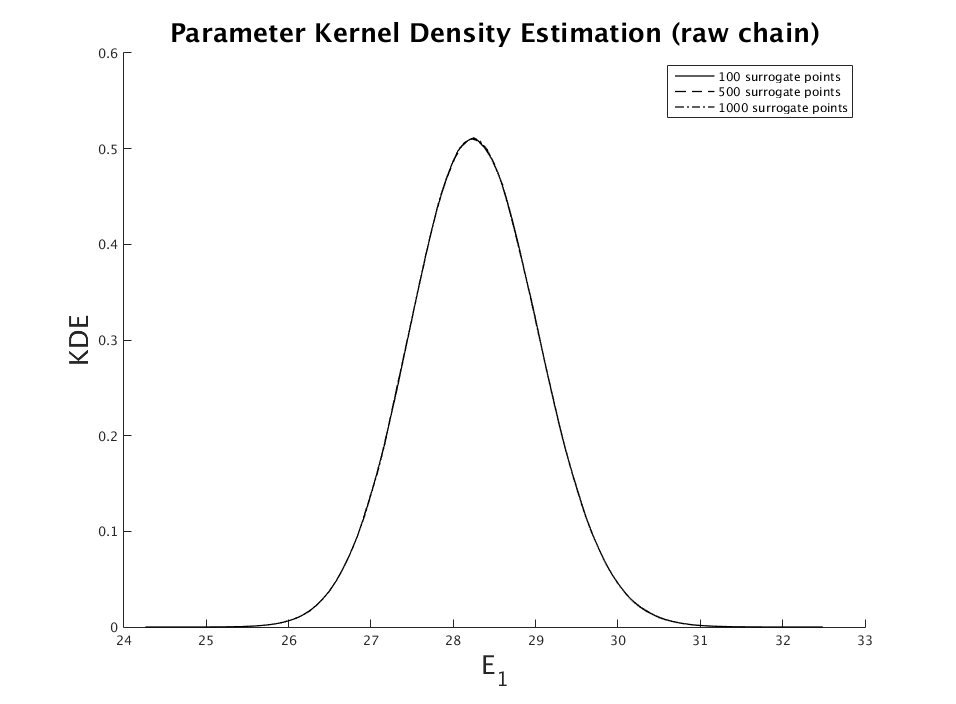
\includegraphics[width=0.45\textwidth]{model_1/conv_surrogate}}
  \caption{Assessing convergence of MCMC sampling and surrogate model.}
\end{figure}


 \begin{figure}[ht]
  \centering
   \subfloat[ Mean  \label{subfig-1:mean_1}]{
        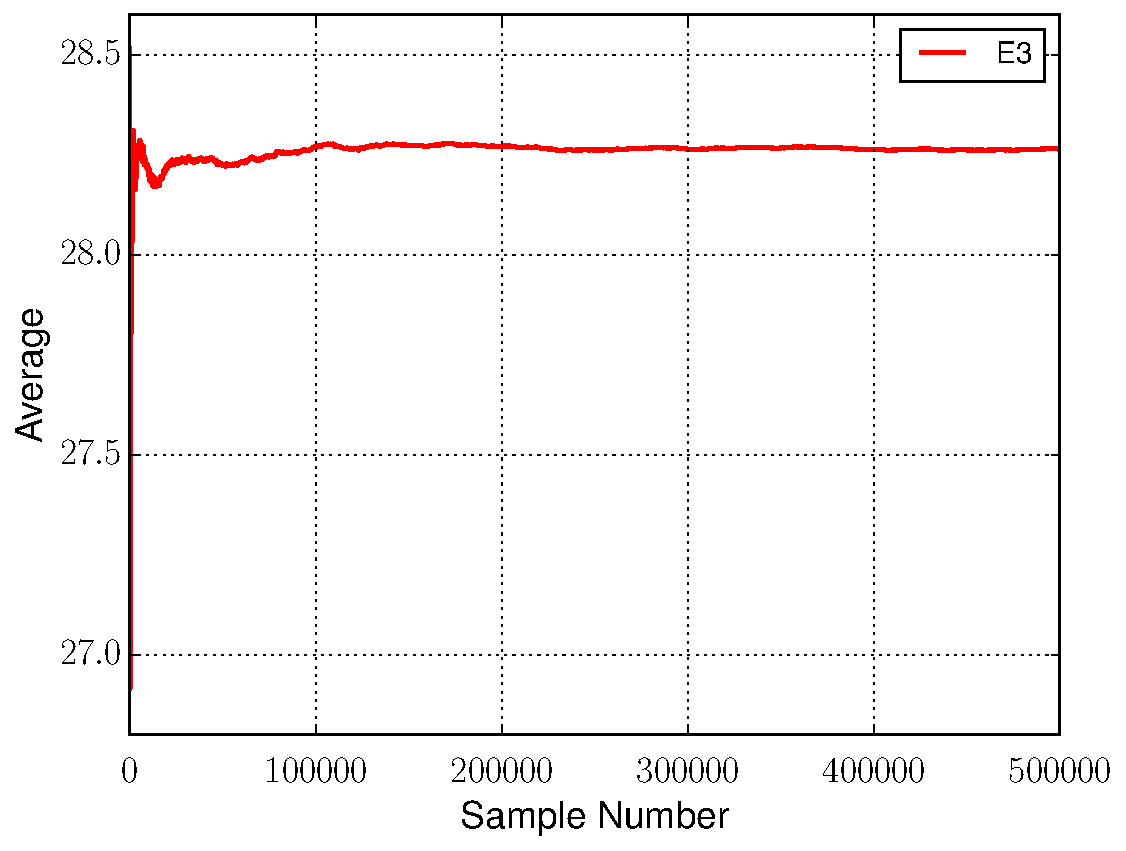
\includegraphics[width=0.45\textwidth]{model_1/M1_running_avg.pdf}
       }
     \quad
\subfloat[Autocorrelation  \label{subfig-2:auto_11}]{
        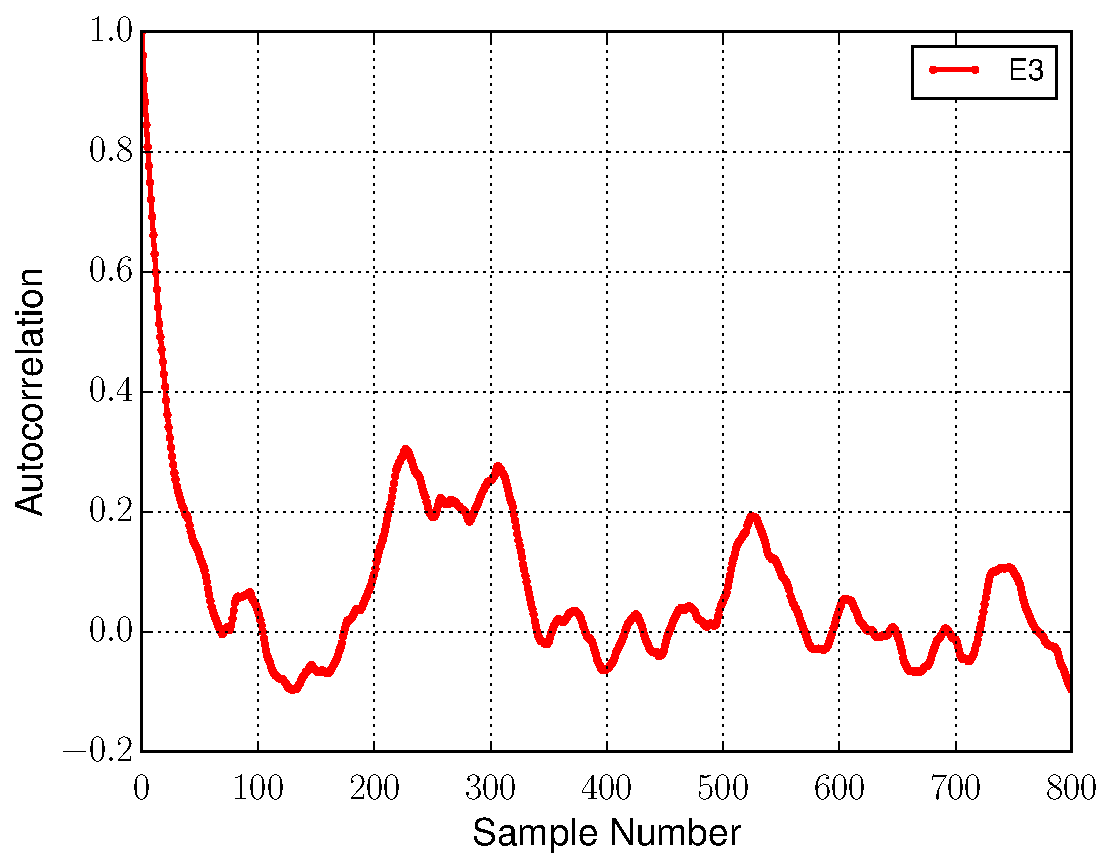
\includegraphics[width=0.45\textwidth]{model_1/M1_autocorr.pdf}
            }
            \caption{Mean and autocorrelation for sample size 1e7}
 \end{figure}

 \begin{figure}[ht]
%  \ContinuedFloat
    \centering
    \subfloat[Histogram of MCMC samples. The red curve shows a Gaussian
      generated by mean and standard deviation of samples.\label{subfig-2:final_e3}]{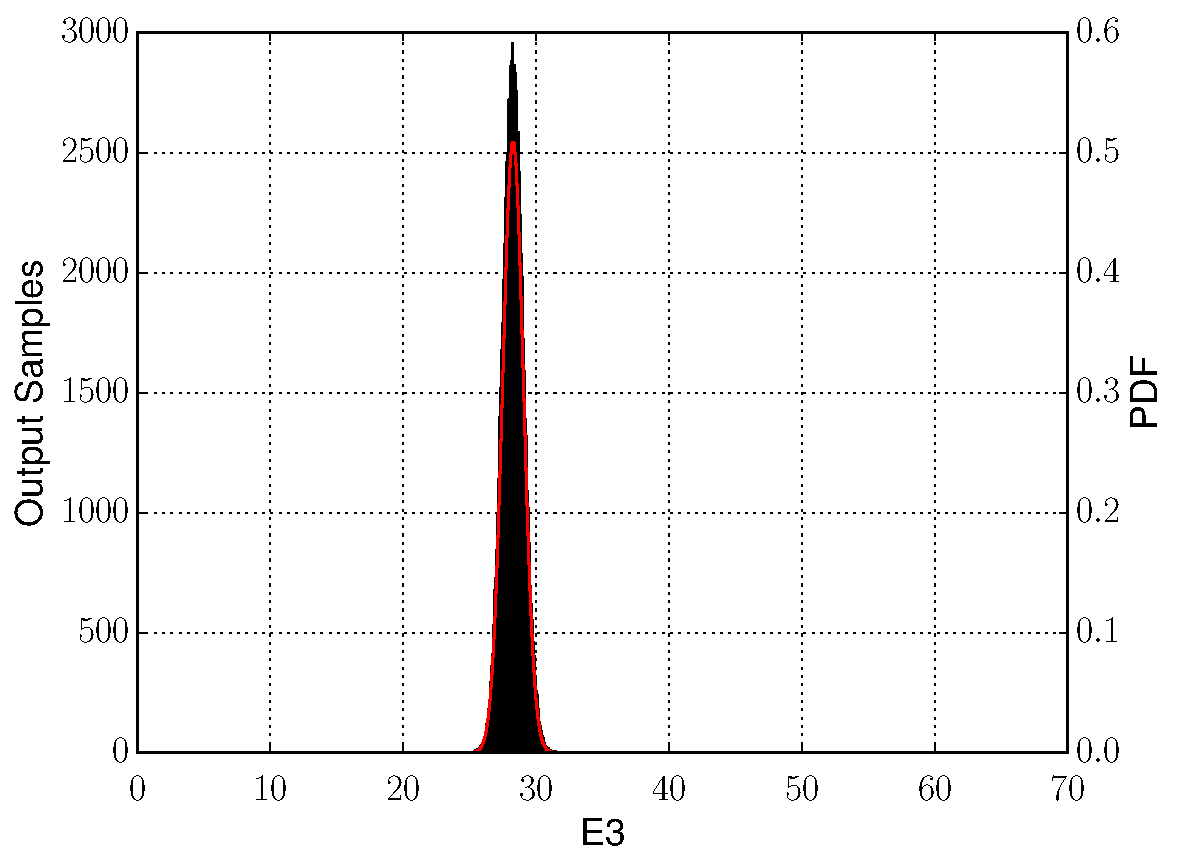
\includegraphics[width=0.45\textwidth]{model_1/E3.pdf}}
      \subfloat[Kernel density estimation.\label{subfig-4:KDE_1}]{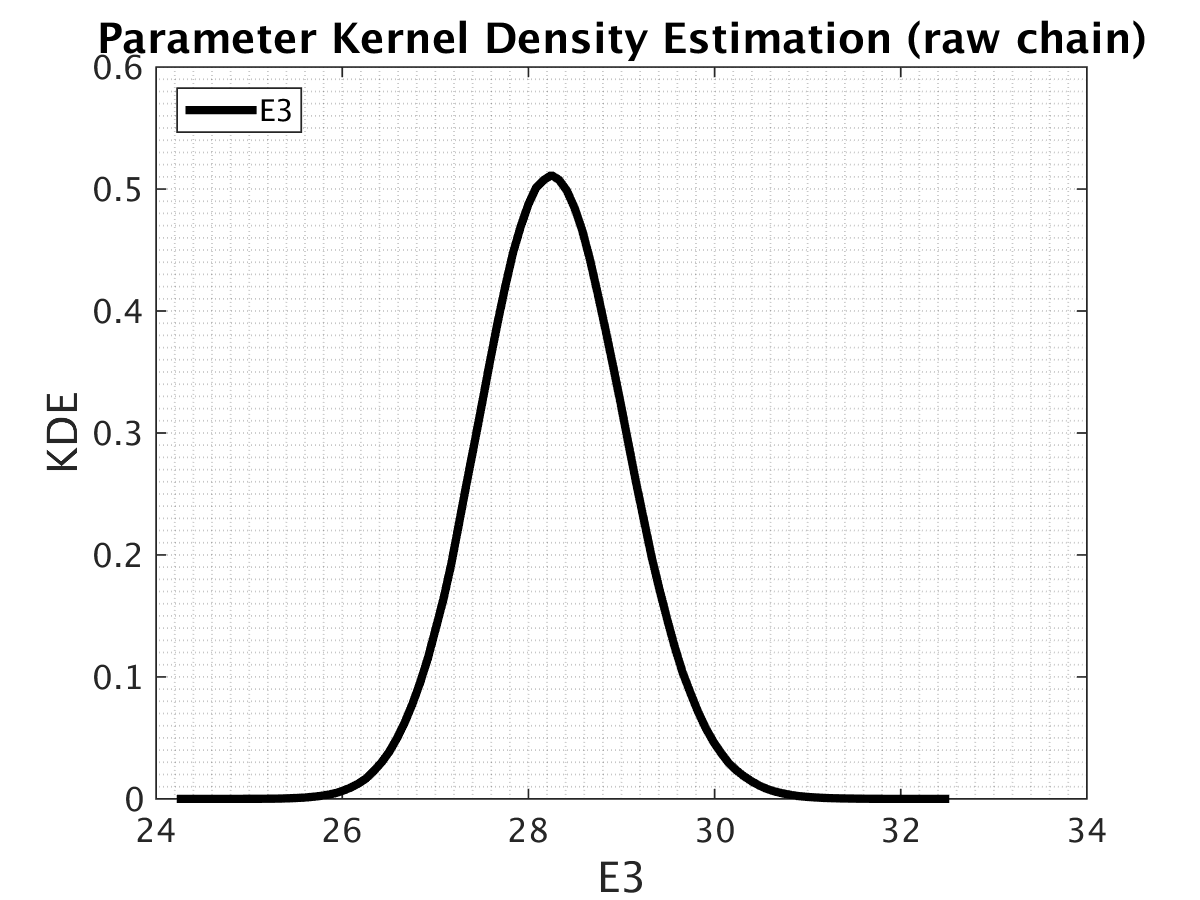
\includegraphics[width=0.45\textwidth]{model_1/simple_ip_kde_raw}}
    \caption{Posterior distribution of $E_3$ following chain thinning.}
 \end{figure}

 \begin{figure}[ht]
   \centering
   \subfloat[ Flame speed for 40 \% ozone. \label{subfig-1:40_1}]{
     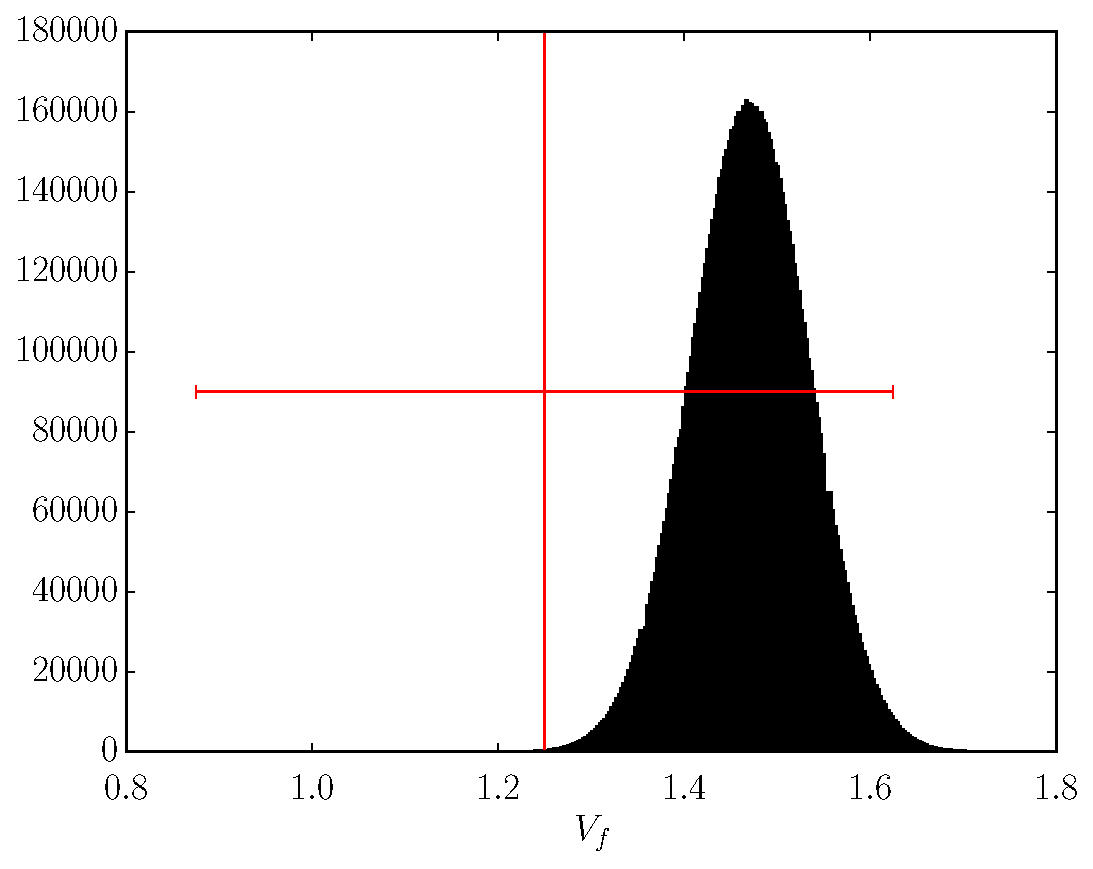
\includegraphics[width=0.4\textwidth]{model_1/flame_40.pdf}
   }
   \subfloat[Flame speed for 46 \% ozone. \label{subfig-2:46_1}]{
     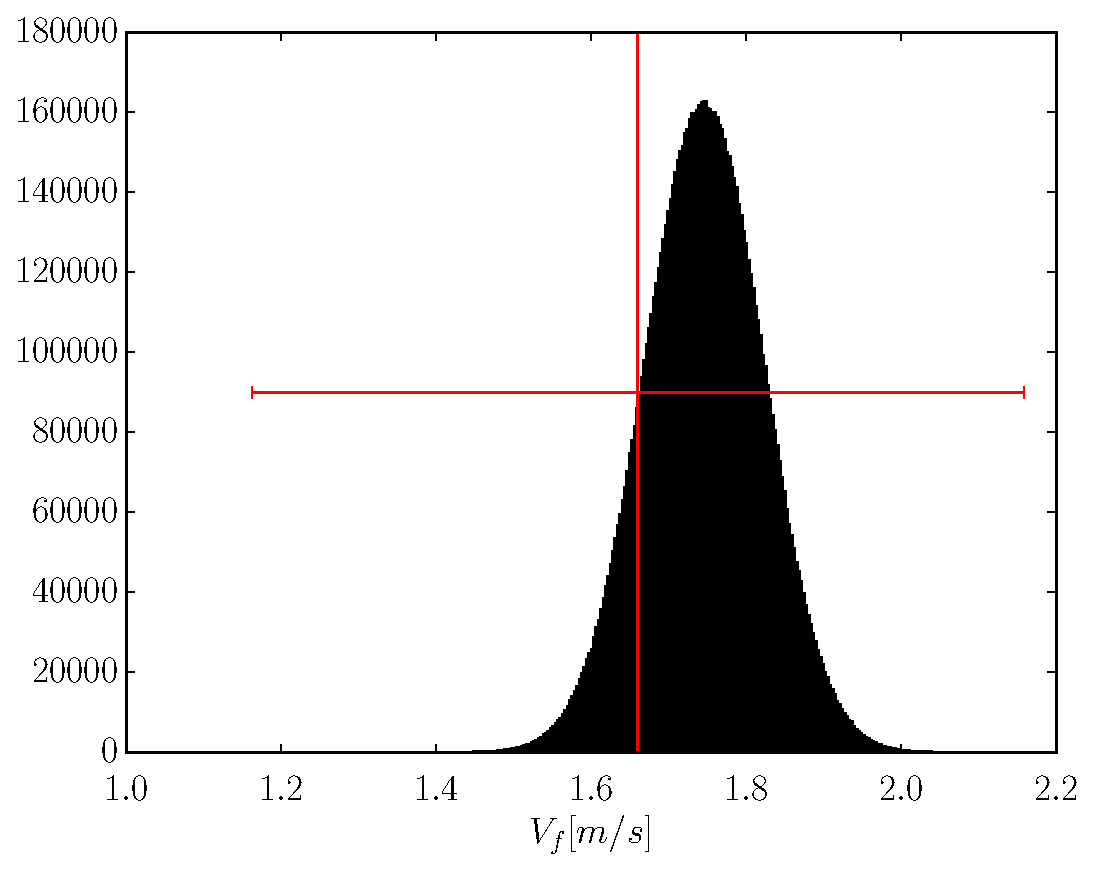
\includegraphics[width=0.4\textwidth]{model_1/flame_46.pdf}
   }

   \subfloat[ Flame speed for 53 \% ozone. \label{subfig-3:53_1}]{
     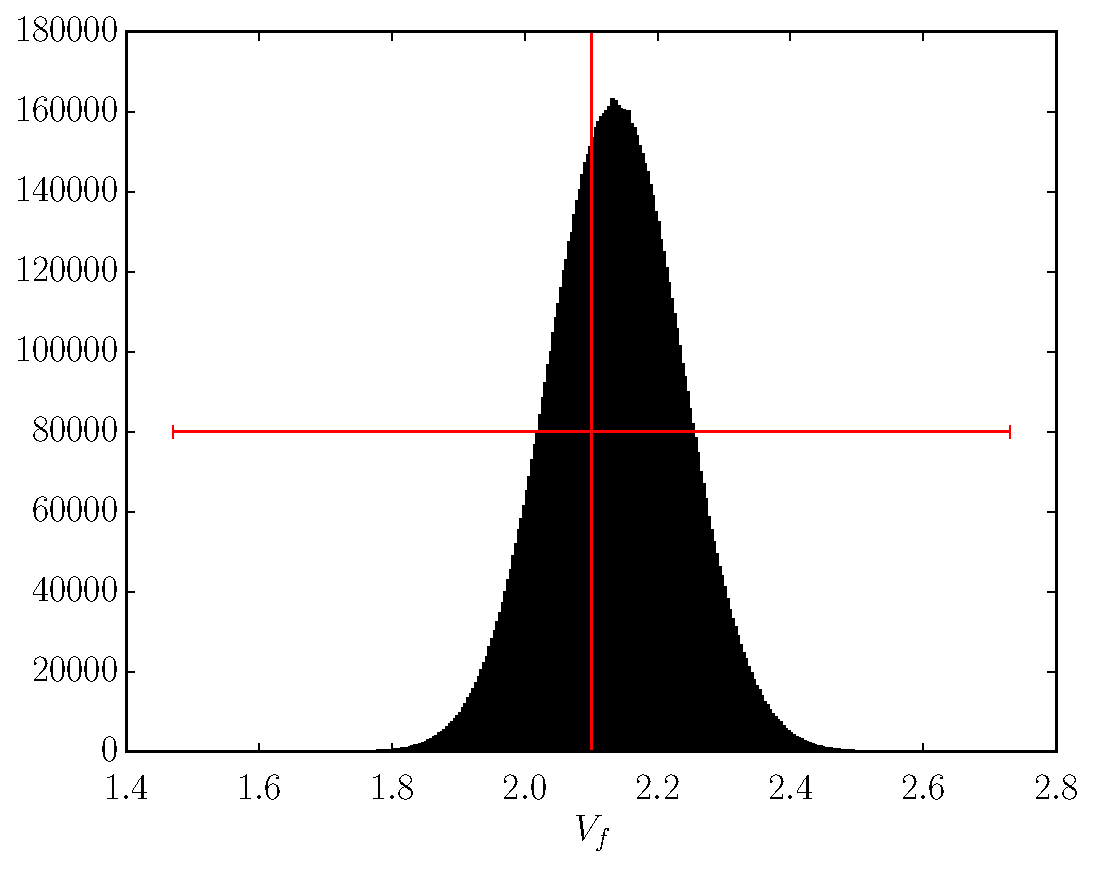
\includegraphics[width=0.4\textwidth]{model_1/flame_53.pdf}
   }
   \subfloat[Flame speed for 75 \% ozone. \label{subfig-4:75_1}]{
     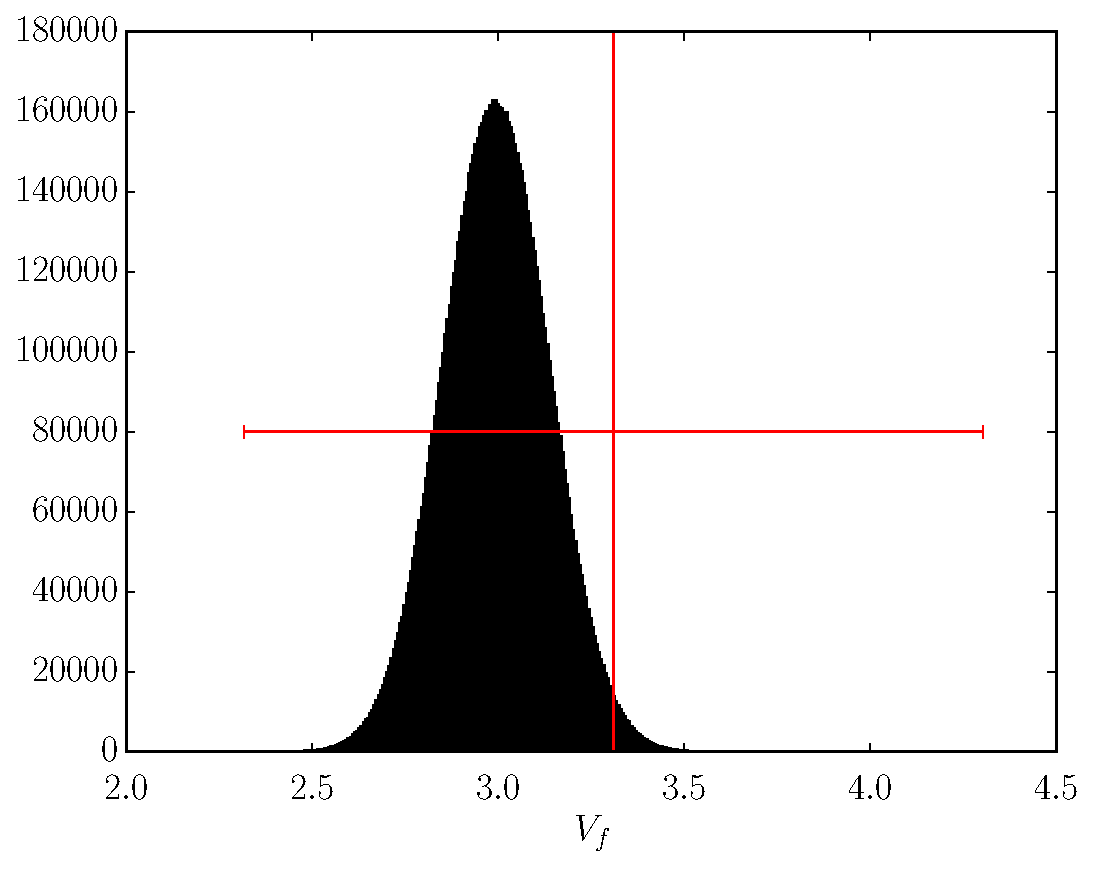
\includegraphics[width=0.4\textwidth]{model_1/flame_75.pdf}
   }

   \subfloat[ Flame speed for 100 \% ozone. \label{subfig-5:100_1}]{
     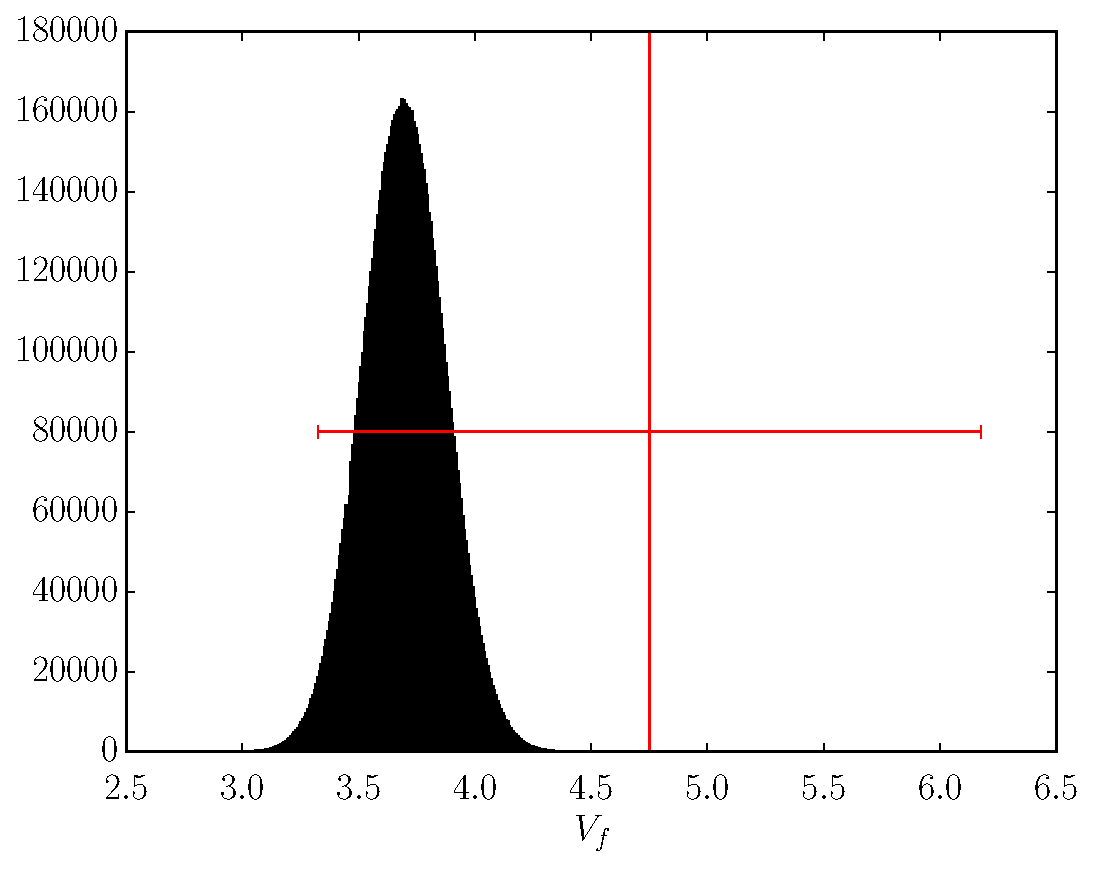
\includegraphics[width=0.4\textwidth]{model_1/flame_100.pdf}
   }
   \caption{Distribution of flamespeed from $E_3$ posterior in order to
     assess quality of parameter fit with experimental data. Red
     vertical line is the data value while the horizontal red line is
     $\pm 30\%$.}
 \end{figure}
